\documentclass[a4paper]{scrreprt}
 
\usepackage[german]{babel}
\usepackage[utf8]{inputenc}
\usepackage[T1]{fontenc}
\usepackage{ae}
\usepackage{graphicx}
 \usepackage[bookmarks,bookmarksnumbered]{hyperref}
 
\begin{document}
 
\title{Entwicklerhandbuch f"ur die Umsetzung des Brettspieles 'Go'}
\author{Harry Flohr (6811837)\\und\\Jan Ole Wellnitz (6796226)}
\maketitle
 \tableofcontents 
 
 \chapter{Strukturen}
\section{Spielfeld}
\label{sec:Spielfeld}
Ein Spielfeld besteht aus 19x19 Felder, auf denen Steine positioniert werden k"onnen. Das Spielfeld wird in dem Programm als eine Liste mit 19 weiteren Listen dargestellt. Diese 19 Listen stehen f"ur die y-Koordinaten des Spielfeldes. Jede dieser 19 Listen enth"alt 19 Positionen, um einen Wert einzutragen. Diese Unterlisten stehen f"ur die x-Koordinaten.\\\\
Wenn an einer Position eine 0 steht, befindet sich kein Stein auf dem Spielfeld. Befindet sich dort eine 1, liegt an der Position ein wei"ser Stein. Bei einer -1, liegt an der Position ein schwarzer Stein.\\
\\Darstellung des Spielstandes in Abbildung 2.3:\\\\
'((0 0 0 0 0 0 0 0 0 0 0 0 0 0 0 0 0 0 0)\\
  (0 0 0 0 0 0 0 0 0 0 0 0 0 0 0 0 0 0 0)\\
  (0 0 0 0 0 0 0 0 0 0 0 0 0 0 0 0 0 0 0)\\
  (0 0 0 0 0 0 0 1 0 0 -1 0 0 0 0 0 0 0 0)\\
  (0 0 0 0 0 0 1 -1 0 0 -1 0 0 0 0 0 0 0 0)\\
  (0 0 0 0 0 0 1 -1 0 1 -1 -1 0 0 0 0 0 0 0)\\
  (0 0 0 0 0 1 1 -1 0 1 1 -1 -1 1 0 0 0 0 0)\\
  (0 0 0 0 0 1 -1 -1 0 1 -1 0 0 0 0 0 0 0 0)\\
  (0 0 0 0 0 1 0 0 0 0 0 0 0 0 0 0 0 0 0)\\
  (0 0 0 0 0 0 0 0 0 0 0 0 1 0 0 0 0 0 0)\\
  (0 0 0 0 0 0 0 0 0 0 0 0 -1 0 0 0 0 0 0)\\
  (0 0 0 0 0 0 0 0 0 0 -1 -1 -1 0 0 0 0 0 0)\\
  (0 0 0 0 0 0 0 0 0 -1 1 1 -1 0 0 0 0 0 0)\\
  (0 0 0 0 1 1 1 1 1 -1 1 1 -1 0 1 1 0 0 0)\\
  (0 0 0 0 1 -1 -1 -1 -1 1 0 1 0 -1 0 -1 1 0 0)\\
  (0 0 0 1 -1 0 -1 1 1 0 0 1 -1 -1 -1 1 0 0 0)\\
  (0 0 0 -1 0 0 -1 1 0 0 0 0 0 0 0 0 0 0 0)\\
  (0 0 0 0 0 0 -1 1 0 0 0 0 0 0 0 0 0 0 0)\\
  (0 0 0 0 0 0 -1 1 0 0 0 0 0 0 0 0 0 0 0))\\

\section{World (Spielzustand)}
\label{sec:World}
Die World setzt sich aus mehreren Informationen zu einer Liste zusammen:

\begin{enumerate}
\item Spielfeld (siehe \ref{sec:Spielfeld})
\item Weltzustand\\
Der Weltzustand gibt an, ob der Client ziehen darf, warten muss oder das Spiel beendet wurde (Zustände: wait, play, lost, won, started, setkilledblack, setkilledwhite, choosedraw, choosepassstatus, choosehandicap, usehandicap).
\item Geschlagene Steine\\
Die bereits geschlagenen Steine werden als Pair '(schwarz . weiß) übergeben.
\item Gepasster Spielzug\\
Hat der vorherige Spieler in seinem Spielzug gepasst und der Spieler an der Reihe passt ebenfalls, ist das Spiel beendet und die Auswertung startet (Gepasst: true/false). 
\end{enumerate}
Als Beispiel eine mögliche World-Darstellung bei der der aktuelle Spieler am Zug ist, 5 schwarze und 8 weiße Steine geschlagen wurden und der vorherige Spieler nicht gepasst hat. Der Spielstand ist zur Übersicht vereinfacht:
\begin{quotation}
 '(play '(spielfeld) '(5 . 8) false)
\end{quotation}
 
\section{Weltzust"ande}
\begin{enumerate}
\item wait: Abwarten
\item play: An der Reihe
\item won: Gewonnen
\item lost: verloren
\item started: Wahl des Spielstarts als neues Spiel oder aus einer Bilddatei
\item setkilledblack: Eingabe der geschlagenen schwarzen Steine bei Spielstart
\item setkilledwhite: Eingabe der geschlagenen wei"sen Steine bei Spielstart
\item choosedraw: Wahl der Zugreihenfolge
\item choosepassstatus: Wahl ob vor Spielstart gepasst wurde
\item choosehandicap: Setzen der H"ohe der Vorgabe
\item usehandicap: Setzen der Vorgabe auf dem Spielfeld
\end{enumerate}
 
\chapter{Module der Software}
 
\section{Bildverarbeitung (go\_bv.rkt)}
Das Modul Bildverarbeitung ist f"ur das Auslesen der Spielfeldbelegung eines Bildes zust"andig. Ein Bild wird in das Modul geladen und dann verarbeitet. Es wird zuerst das Spielbrett aus dem Bild extrahiert und in ein Schwarz-Wei"s-Bild gewandelt. Die Graustufen stellen die Anteile der blauen Farbe in dem originalen Bild dar. Das Bild wird anschlie"send noch verwaschen, um die Spielfeldlinien und Reflexionen leichter von den Spielsteinen unterscheiden zu k"onnen.\\\\
In diesem Bild wird die Koordinaten des ersten Spielfeldes (oben links) gesucht. An dieser Koordinate wird geschaut, ob die Schwellenwerte f"ur einen wei"sen oder schwarzen Stein getroffen wird. Diese "Uberpr"ufung wird an insgesamt neun Stellen pro Koordinate vorgenommen. Es wird quadratisch um die Koordinate kontrolliert (siehe Abb. 2.1). 
\begin{figure}[ht]
\centering 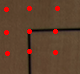
\includegraphics[width=0.3\textwidth]{images/koordinate}
\caption{Suchemuster an Koordinate}
\end{figure}
\\\\
Dieser Prozess wird an jeder m"oglichen Koordinate f"ur einen Stein durchgef"uhrt und so eine Spielfeldbelegung, wie in \ref{sec:Spielfeld} beschreiben, erstellt. Die Koordinaten werden anhand zweier Schrittweiten (in x - und y-Richtung) ermittelt. Ist das ganze Spielfeld kontrolliert, hat das Modul die vollst"andige Spielfeldbelegung des Bildes projiziert.
\newpage

\section{Spielbrett zeichnen (go\_draw\_board.rkt)}
Das Modul go\_draw\_board.rkt ist f"ur die Anzeige des gesamten User-Interfaces zust"andig.\\\\
Es zeichnet zum einen aus einer g"ultigen Spielfeldbelegung (\ref{sec:Spielfeld}) das belegte Spielbrett. Zuerst wird das Grundbrett gezeichnet. Anschlie"send werden die Listen des Spielstandes ausgelesen und die ben"otigten Steine auf das Spielfeld gezeichnet. Die Leserichtung der Listen erfolgt von oben links nach unten rechts.\\

\begin{figure}[ht]
\centering 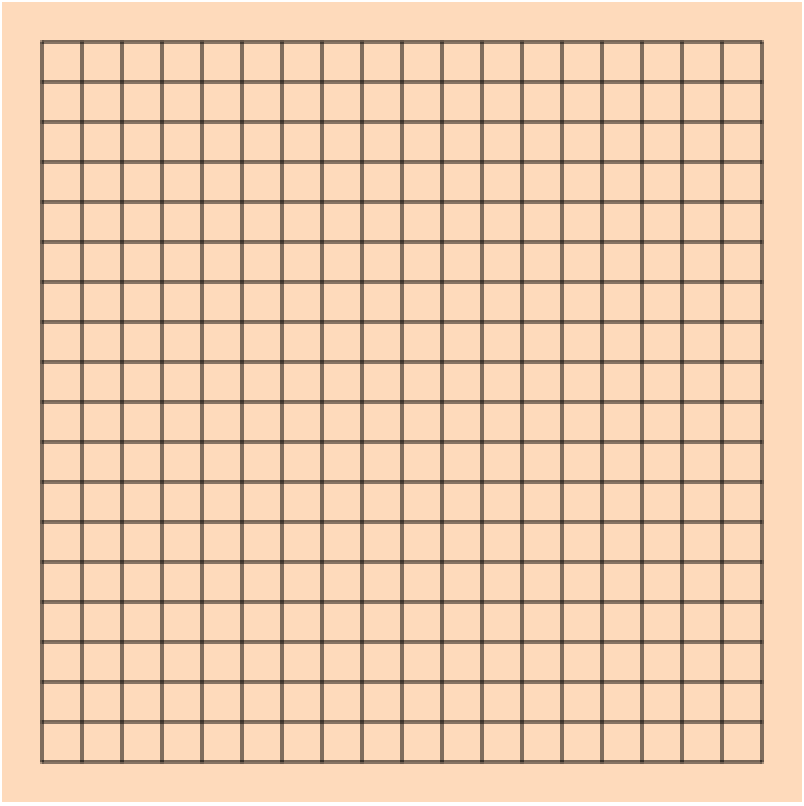
\includegraphics[width=0.3\textwidth]{images/emptyBoard}
\caption{Leeres Spielfeld}
\end{figure}

\begin{figure}[ht]
\centering 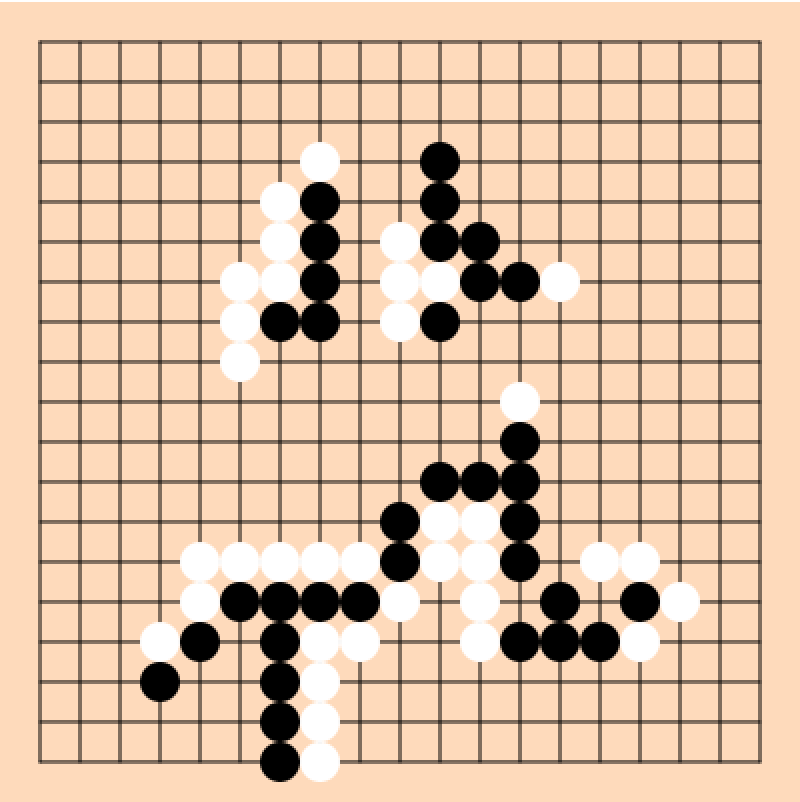
\includegraphics[width=0.3\textwidth]{images/board}
\caption{Belegtes Spielfeld}
\end{figure}
\newpage 

Zudem zeichnet das Modul beim Start eines Spieles die ben"otigten Auswahloptionen, die der Benutzer vor dem Starten eingeben muss. Das kann zum einen "uber das Darstellen einer Auswahlfl"ache (Abb. 2.4) geschehen, auf die der Benutzer klicken muss. Zum anderen aber auch eine Aufforderung zur Eingabe von Zahlen "uber die Tastatur (Abb. 2.5). 
\begin{figure}[ht]
\centering 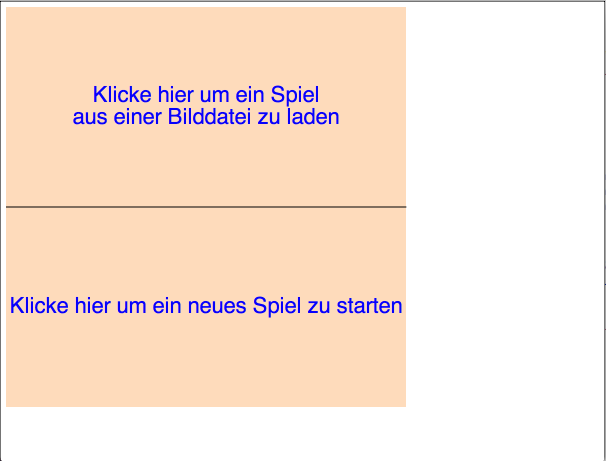
\includegraphics[width=0.5\textwidth]{images/Optionsauswahl}
\caption{Auswahl "uber Optionsfelder}
\end{figure}

\begin{figure}[ht]
\centering 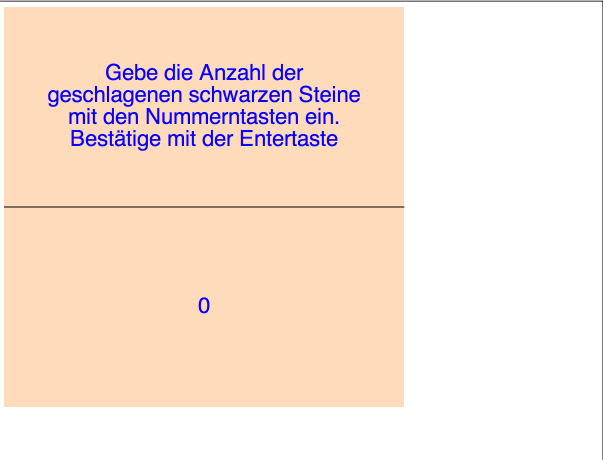
\includegraphics[width=0.5\textwidth]{images/Zahleneingabe}
\caption{Zahleneingabe}
\end{figure}
\newpage
Nach Eingabe aller Parameter erstellt die Komponente das User-Interface f"ur das Spielen selbst. Dazu geh"oren das Spielfeld, Spielstatus des Spielers,die erzielten Punkte und Buttons (f"ur Passen oder ein neues Spiel starten) (Abb. 2.6).

\begin{figure}[ht]
\centering 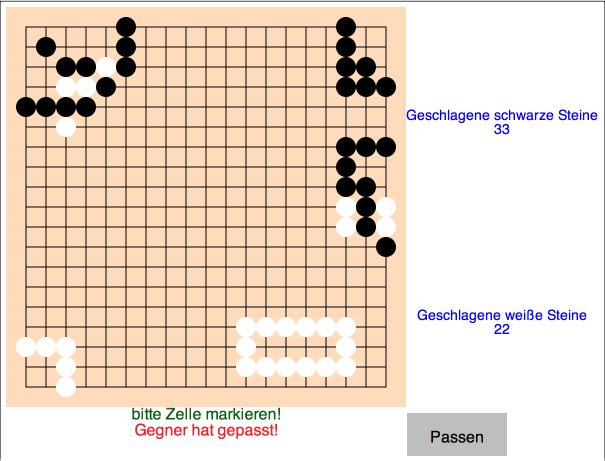
\includegraphics[width=0.5\textwidth]{images/Spielfeld}
\caption{Das Spielfeld w"ahrend des Spiels}
\end{figure}

Alle Darstellung des User-Interfaces k"onnen "uber die Schnittstellen des Moduls angezeigt werden. Soll eine z. B. Eingabeoption erstellt werden, muss dazu eine neue Funktion erstellt werden und als Schnittstelle bereit gestellt werden. Um bestehende Darstellungen zu "andern, m"ussen die entsprechenden Funktionen in diesem Modul angepasst werden.

\newpage

\section{Spielclient (go\_client.rkt)}
Der Spielclient steuert die Kommunikation des Spielers mit dem Server. Mit dem Spielclient kann  auf zwei verschiedene Arten ein Spiel gestartet werden. Es kann ein komplett neues Spiel gestartet werden und es kann ein Spielstand mit einem Bild-Spielstand gestartet werden. Bei dem Start aus einem Bild-Spielstand fragt der Client ab, wie viele Steine bereits geschlagen wurden, welche Farbe der Spieler hat, ob ein Spieler gepasst hat und welcher Spieler am Zug ist. Diese Informationen werden dann zu dem Server geschickt und dieser initialisiert den ersten Spielstand (\ref{sec:World}). Die Funktionen zum zeichnen der Auswahloptionen und Eingaben stammen aus dem go\_draw\_board.rkt Modul.\\\\
Ebenfalls ist der Spielclient f"ur die Erstellung des Interfaces zust"andig. "Uber dieses zeigt er den Spielern w"ahrend eines Spiels den aktuellen Spielstand an, ob sie an der Reihe sind, die Anzahl der geschlagenen Steine, ob der Gegner gepasst hat, sie einen ung"ultigen Zug vorgenommen haben und wer gewonnen hat. Auch die Buttons zum Passen oder f"ur das Starten eines neuen Spiels, werden angezeigt. Diese Anzeige wird "mit Hilfe das  go\_draw\_board.rkt Modul erstellt.\\\\ 
Die Hauptaufgabe des Clients ist aber die Entgegennahme von Benutzereingaben. Der Client nimmt Click-Events und Tastatureingaben entgegen, leitet sie zum Server weiter, empf"angt das Ergebnis und stellt das Ergebnis dar. So kann der Benutzer "uber den Client ein Spiel starten, die Spiel-Parameter eingeben, das Spiel bis zum Ende durchf"uhren und anschlie"send ein neues Spiel starten.

\section{Spielserver (go\_server.rkt)}
Der Spielserver leitet das Spiel. Zu Beginn erh"alt der Server die Information, ob er ein neues Spiel starten oder ein Spiel aus einem Bild laden soll. Der Server l"adt das Bild und ermittelt den Spielstand. Der Server schickt dann ggf. eine Abfrage f"ur die weiteren ben"otigten Informationen an den Client. Diese sind bei einem neuen Spiel die Vorgabe und bei einem Spielstand aus einem Bild die geschlagene Steine, der Spieler, der am Zug ist, und ob der vorherige Spieler gepasst hat. Anschlie"send sendet der Server den vollst"andigen Startzustand an die Clients.\\\\
Eine weitere Aufgabe w"ahrend des gesamten Spieles ist die Verwaltung des Spielstandes (\ref{sec:World}) und welcher Spieler am Zug ist. Ebenfalls pr"uft der Server die "ubermittelten Spielz"uge der Spieler auf ihre G"ultigkeit und teilt den Spielern ggf. mit, dass der Spielzug nicht zul"assig ist. Bei zul"assigen Z"ugen passt der Server den Spielstand (\ref{sec:World}) an und "ubermittelt den vollst"andig erstellten Spielstand an die Clients.\\\\ 
Nach Beendigung eines Spieles, ermittelt der Server den Gewinner und teilt den Spielern (Clients) den Gewinner mit.

\section{Spiellogik (go\_logic.rkt)}
In dem Modul go\_logic.rkt ist die Spiellogik implementiert. Diese kann in drei verschieden Aufgaben unterteil werden.

\begin{enumerate}
\item Vorgaben machen:\\
Wenn bei dem Start eines neuen Spiels eine Vorgabe gew"ahrt wird, kann der Spieler vor Spielbeginn die angegebene Anzahl Steine setzen.

\item Stein setzen:\\
Wenn ein Stein gesetzt wird, muss gepr"uft werden, dass dieser keinen Selbstmord begeht (Abb. 1.7). Das w"urde bedeuten, dass dieser Stein und ggf. seine anliegende Struktur durch das Setzen dieses Steines zerst"ort wird.

\begin{figure}[ht]
\centering 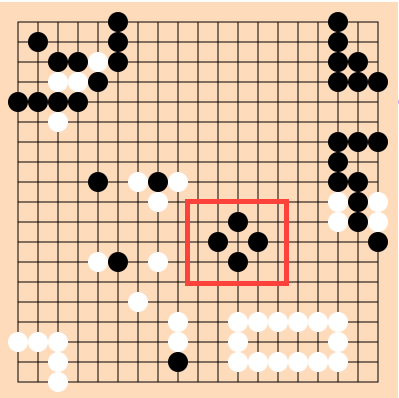
\includegraphics[width=0.3\textwidth]{images/Selbstmord}
\caption{Selbstmord - Wei"ser Stein darf nicht gesetzt werden}
\end{figure}

Dieser Zug ist nur erlaubt, wenn mit diesem Zug Steine des Gegners geschlagen werden und so der Stein und ggf. seine Struktur neue Freiheiten erhalten.

Wenn ein Stein normal gesetzt wird, kann das Setzen zur Folge haben, dass durch diesen Zug eine Struktur des Gegners zerst"ort wird. Wenn dieser Fall eintritt m"ussen alle geschlagenen Steine von dem Spielfeld entfernt werden und die Punkte werden dem Spieler gut geschrieben.
\begin{figure}[ht]
\centering 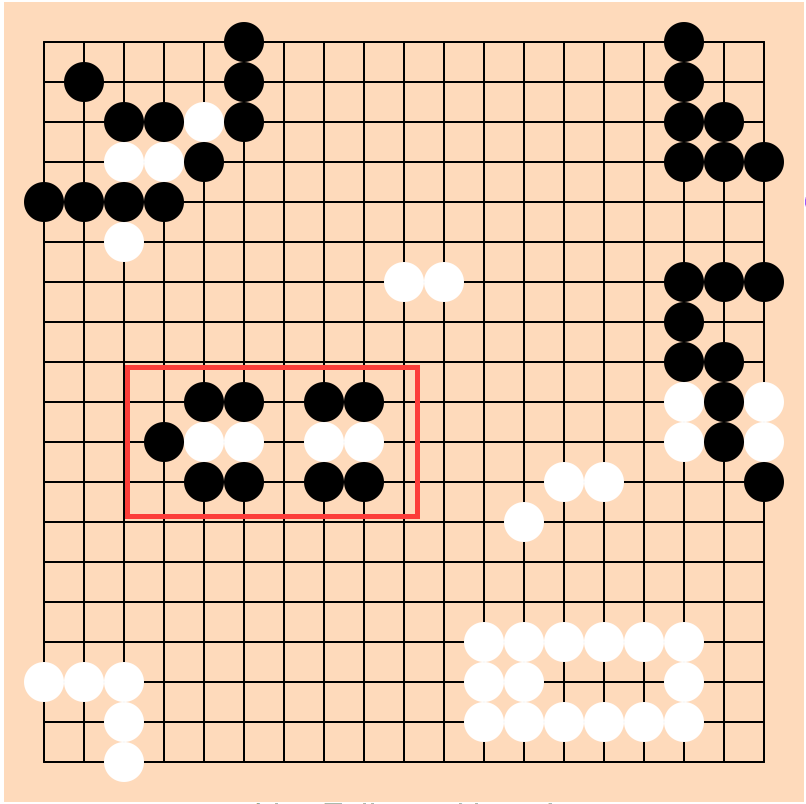
\includegraphics[width=0.3\textwidth]{images/Vor-Kill}
\caption{Spielbrett vor dem Schlagen der Steine}
\end{figure}

\begin{figure}[ht]
\centering 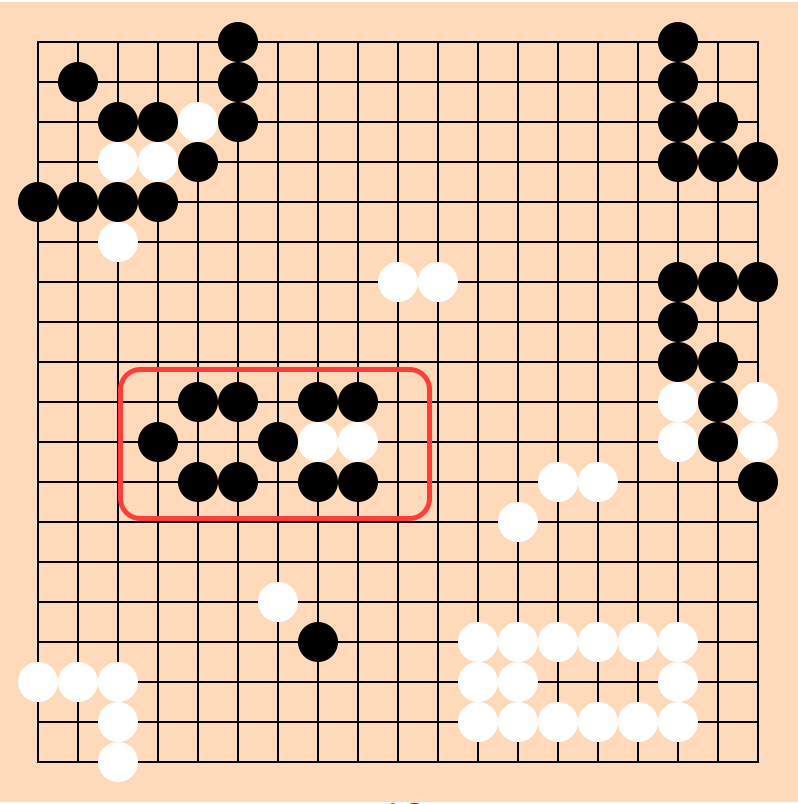
\includegraphics[width=0.3\textwidth]{images/Nach-Kill}
\caption{Spielbrett nach dem Schlagen der Steine}
\end{figure}
\item Auswertung:\\
Nachdem beide Spieler nacheinander gepasst haben, ist das Spiel beendet. Dann startet die Auswertung. Bei der Auswertung m"ussen eroberte Gebiete gefunden werden. Das sind Fl"achen auf denen kein Stein liegt, die aber von einem Spieler eingeschlossen sind. Wenn ein Spieler eine freie Fl"ache erobert hat, erh"alt dieser die Anzahl an freien Positionen sowie die Anzahl der gegnerischen Steine in diesem Gebiet. Ein erobertes Gebiet ist in Abb. zu sehen. Nachdem alle Fl"achen "uberpr"uft sind, wird die Anzahl der erzielten Punkte auf die bereits erzielten Punkte aufaddiert.

\begin{figure}[ht]
\centering 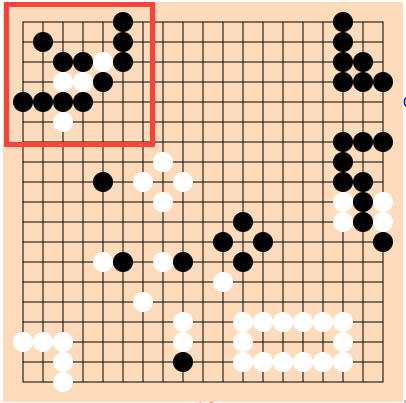
\includegraphics[width=0.3\textwidth]{images/Gebiet}
\caption{Gebiet von Schwarz eingenommen - 13 freie Fl"achen + 3 geschlagene wei"se Steine}
\end{figure}

\end{enumerate}
Diese drei Hauptaufgaben k"onnen "uber Schnittstellen ausgef"uhrt werden. "Anderungen in der Spiellogik bzw. Erweiterungen sind demzufolge in diesem Modul zu erledigen.

 \chapter{Schnittstellen}
 \section{Bildverarbeitung}
\begin{enumerate}
\item (board-state):\\
Das Modul bietet diese Funktion, um die Belegung eines Spielfeldes aus einem Bild heraus auszulesen. Der Dateipfad des Bildes ist in dem Modul selbst hinterlegt. Durch den Aufruf liefert die Funktion die Belegung des Spielfeldes, wie in \ref{sec:Spielfeld} beschrieben, zur"uck.
\end{enumerate}

\section{Spielbrett zeichnen}

\begin{enumerate}
\item (draw-board-with-score world):\\
Die Funktion zeichnet das User-Interface w"ahrend des Spieles. Dazu geh"oren das Spielfeld mit der aktuellen Belegung, Anzahl der geschlagenen Steine, welcher Spieler am Zug ist, Passstatus des Gegners sowie ein Button zum Passen oder nach der Auswertung f"ur den Start eines neuen Spieles. Auf dem Spielfeld kann anschlie"send auf die gew"unschte Stelle f"ur einen Steine ausgew"ahlt werden, der Client verarbeitet diese Eingabe und schickt sie zu dem Server.

\item (start-field):\\
Diese Funktion zeichnet das User-Interface f"ur die Auswahl, ob eine Datei aus der Bilddatei gestartet werden soll oder ob ein komplett neues Spiel gestartet wird. Dazu werden zwei Auswahlbereiche gezeichnet, die der Benutzer per Mausklick ausw"ahlen kann.

\item (choose-color-field):\\
Diese Funktion zeichnet das User-Interface f"ur die Auswahl, mit welcher der ausw"ahlende Spieler spielt. Dazu werden zwei Auswahlbereiche gezeichnet, die der Benutzer per Mausklick ausw"ahlen kann.

\item (choose-killed-black-stones killed-stones):\\
Diese Funktion zeichnet das User-Interface f"ur die Eingabe, wie viele schwarze Steine bereits geschlagen worden sind. Dazu wird ein Infotext sowie eine Eingabeanzeige gezeichnet. Die Eingabe erfolgt per Tastatur. Nach jeder Eingabe wird die Anzeige aktualisiert.

\item (choose-killed-white-stones killed-stones):\\
Diese Funktion zeichnet das User-Interface f"ur die Eingabe, wie viele wei"se Steine bereits geschlagen worden sind. Dazu wird ein Infotext sowie eine Eingabeanzeige gezeichnet. Die Eingabe erfolgt per Tastatur. Nach jeder Eingabe wird die Anzeige aktualisiert.

\item (draw-final-score world):\\
Diese Funktion zeigt den Gewinner sowie erreichte Punktzahl beider Spieler an.

\item (choose-handicap handicap):\\
Diese Funktion zeichnet das User-Interface f"ur die Eingabe, wie viele Steine ein Spieler als Vorlage legen darf. Dazu wird ein Infotext sowie eine Eingabeanzeige gezeichnet. Die Eingabe erfolgt per Tastatur. Nach jeder Eingabe wird die Anzeige aktualisiert.

\item (set-handicap world):\\
Diese Funktion erm"oglicht das Setzen der Vorgabe. Dazu werden das Spielfeld und die Anzahl der Vorgabe angezeigt. Nach jedem gesetzten Stein wird die Anzeige aktualisiert.

\item (choose-draworder-field):\\
Diese Funktion zeichnet das User-Interface f"ur die Auswahl, welcher Spieler zuletzt am Zug war. Dazu werden zwei Auswahlbereiche gezeichnet, die der Benutzer per Mausklick ausw"ahlen kann.

\item (choose-passstatus):\\
Diese Funktion zeichnet das User-Interface f"ur die Auswahl, ob ein Spieler im letzten Zug vor der Fotoaufnahme gepasst hat. Dazu werden zwei Auswahlbereiche gezeichnet, die der Benutzer per Mausklick ausw"ahlen kann.
\end{enumerate}

\section{Spielclient}

\begin{enumerate}
\item (receive w m):\\
Der Spielclient erh"alt "uber die von dem Universe-Paket gelieferten Funktion seinen Spielstand (\ref{sec:World}). In dem Parameter w befindet sich der alte Weltzustand und in dem Parameter m der neue Weltzustand. Der neue Weltzustand m wird zuerst "uberpr"uft. Ist er g"ultig wird dieser angezeigt, ist er es nicht, wird der alte Weltzustand gew"ahlt.

\item (make-package w m):\\
Der Spielclient kann mittels der Funktion (make-package w m) mit dem Server kommunizieren. So kann der Spielclient mit dem Parameter w seine aktuelle Welt senden und in dem Parameter m weitere Informationen verpacken. Zum Beispiel wird dort angegeben an welcher Position der Spieler seinen Stein gesetzt hat.

\end{enumerate}

\section{Spielserver}
\begin{enumerate}
\item (make-mail to content):\\
Der Spielserver kann mit der Funktion make-mail Informationen an den Client senden. In dem Parameter to wird das Ziel des Aufrufes festgelegt. In dem content befindet sich der aktuelle Spielstand (\ref{sec:World}).

\item (handle-messages univ wrld m):\\
Der Server kann mit der Funktion handle-messages Daten von den Clients empfangen. In dem Parameter univ befindet sich das Universum selbst. In wrld befindet sich die von dem Client gesendete World und in dem Parameter m die Aktion, die der Client gerne ausf"uhren m"ochte. Das kann z. B. das Setzen eines Steines sein. Dann befindet sich in m die Funktion 'set sowie die x- und y-Koordinaten der Position, an der der Stein gesetzt werden soll. Ebenfalls k"onnen sich in dem Parameter m die Informationen f"ur den Spielstart befinden. Wie z. B. die Vorgabe oder die geschlagenen Steine. 

\item (add-world univ wrld):\\
Mit der Funktion add-world kann sich ein Client bei dem Server anmelden. Dazu wird das Universum (univ) sowie die World (wrld) ben"otigt. Wenn zwei Clients angemeldet sind, werden weitere Clients abgewiesen.
\end{enumerate}

\section{Spiellogik}
\begin{enumerate}

\item (do-set univ wrld m):\\
Die do-set Funktion erm"oglicht das setzen eines Steines. Wenn ein Spieler einen Stein setzt, wird gepr"uft, ob der Zug zul"assig ist und ob und wie viele Steine von dem Gegner geschlagen wurden. Geschlagene Steine werden ebenfalls von dem Spielbrett entfernt.

\item (do-handicap univ wrld m):\\
Die do-handicap Funktion erm"oglicht das setzen der Vorgabe. Ein Spieler kann so oft einen Stein hintereinander setzen bis seine Vorgaben verbraucht sind. 

\item (calc-score board):\\
Die calc-score Methode ermittelt am Ende des Spieles anhand des Spielfeldes das Endergebnis. Dazu werden eroberte Fl"achen gesucht und ausgewertet. Jede freie Position sowie jeder gegnerische Stein in einem eroberten Gebiet sind ein Punkt f"ur den Eroberer. Diese Funktion liefert ein Pair mit den erzielten Punktet zur"uck. (schwarz . wei"s)
\end{enumerate}

 \chapter{Paketstruktur}
 \begin{figure}[ht]
\centering 
\includegraphics[width=1.1\textwidth]{images/Paketstruktur}
\caption{Paketstruktur}
\end{figure}

\chapter{Programmabl"aufe}
\section{Programmablauf}
\begin{figure}[ht]
\centering 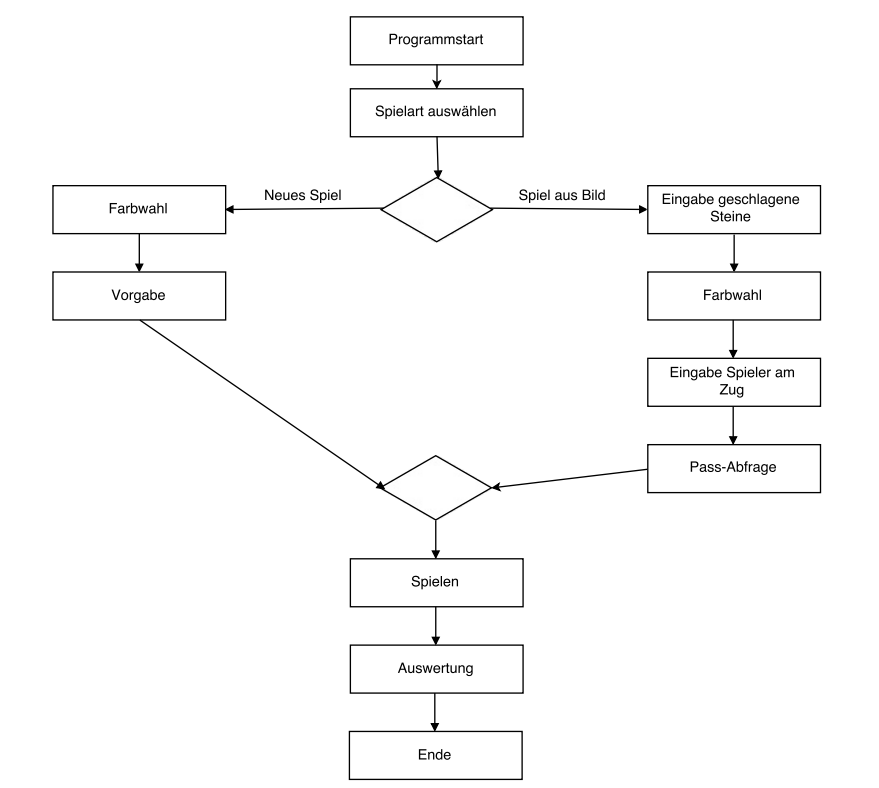
\includegraphics[width=1.1\textwidth]{images/Ablauf}
\caption{Ablaufdiagramm des Programmes}
\end{figure}

\section{Stein setzen}
\label{sec:SteinSetzen}
\begin{figure}[ht]
\centering 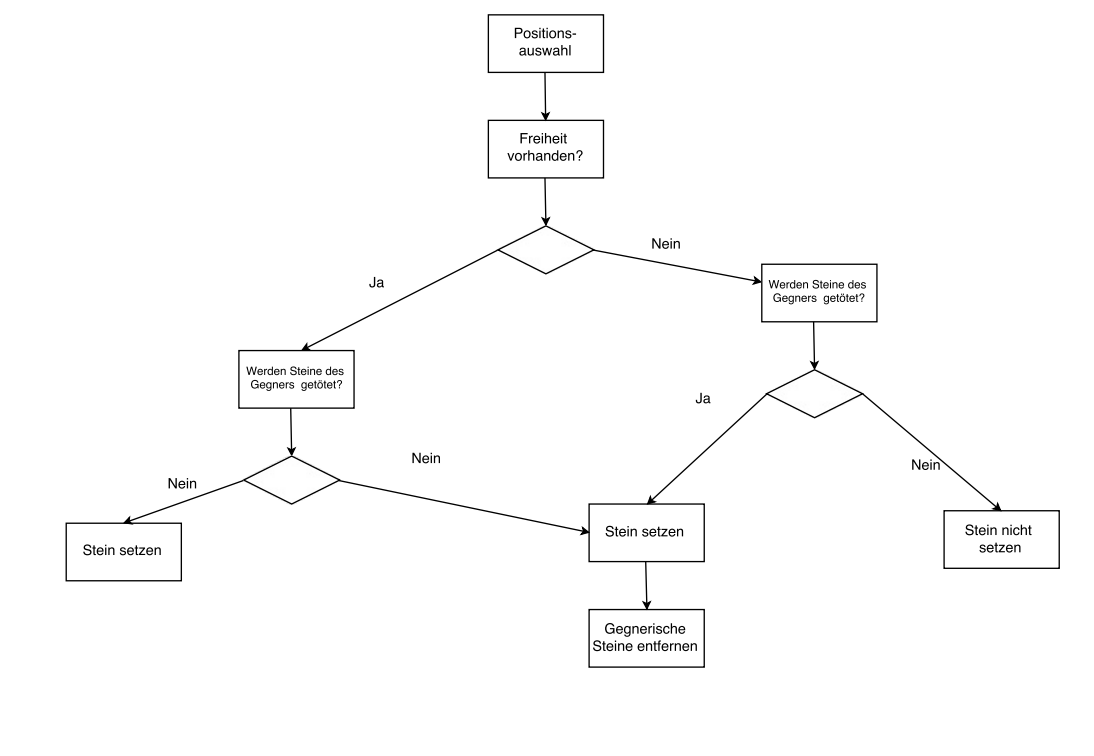
\includegraphics[width=1.1\textwidth]{images/SteinSetzenAblauf}
\caption{Ablaufdiagramm f"ur das Setzen eines Steines}
\end{figure}
Wenn ein Spieler einen Stein setzt muss die g"ultigkeit dieses Zuges gepr"uft werden. Wenn keine Freiheit direkt bei dem zu setzenden Stein zu finden ist, m"ussen alle direkten Steine der gleichen links, rechts, oben und unten von dem gesetzten Stein auf vorhandene Freiheiten "uberpr"uft werden. Diese benachbarten Steine werden als Startpunkte genommen. Von diesen werden weitere benachbarte Steine der gleichen Farbe gesucht. Diese Suche wird so lange fortgesetzt bis eine Freiheit gefunden wird. Wird eine Freiheit gefunden, kann der Stein gesetzt werden. Wird keine Freiheit gefunden, ist der Zug ung"ultig, weil der Spieler die eigene Struktur mit diesen Zug selbst schlagen w"urde. Diesen Zug nennt man dann Selbstmord und das ist nicht erlaubt.\\\\
Dieser Zug ist nur zugelassen, wenn man mit diesen Zug Steine des Gegners schlagen w"urde. Dazu muss der gleiche Prozess nur mit benachbarten Steinen der gegnerischen Farbe durchlaufen werden. Wird keine Freiheit gefunden, werden die Steine des Gegners geschlagen und die eigene Struktur erh"alt neue Freiheiten.\\\\
Die Pr"ufung auf geschlagene Steine des Gegners wird ebenfalls durchgef"uhrt, wenn ein Zug sofort als g"ultig erkannt wird. Das hei"st, dass der Zug keinen Selbstmord hervorruft, aber Steine schl"agt. Das hei"st, dass bei jedem regul"ar gesetzten Steine die benachbarten gegnerischen Strukturen auf Freiheiten "uberpr"uft werden. Findet sich bei einer Struktur wiederum keine Freiheit, werden die Steine entfernt und die Punkte werden dem setzenden Spieler hinzugef"ugt.

\begin{figure}[ht]
\centering 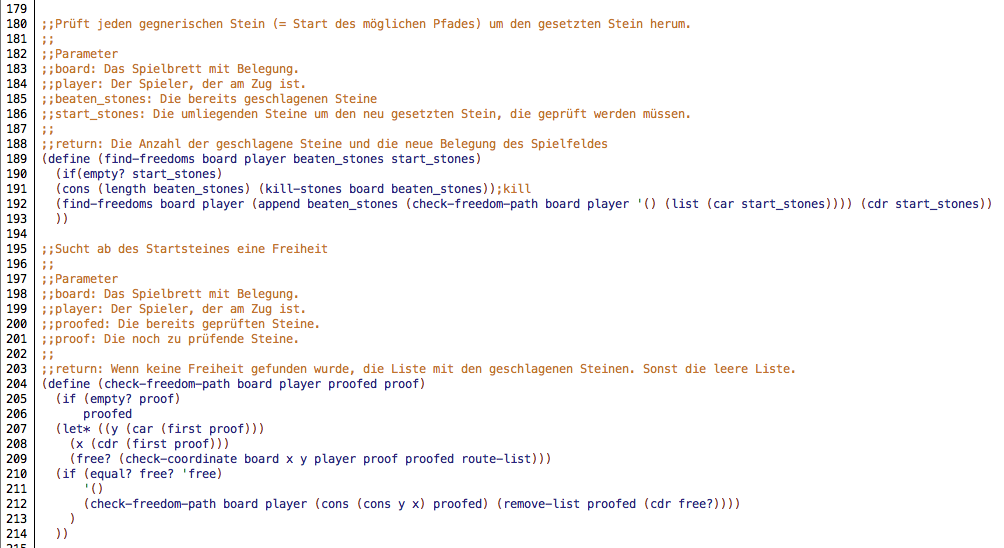
\includegraphics[width=1\textwidth]{images/Freiheit_code}
\caption{Funktionen f"ur das Suchen von Freiheiten benachbarter Steinen}
\end{figure}
\newpage
\section{Auswertung}
\begin{figure}[ht]
\centering 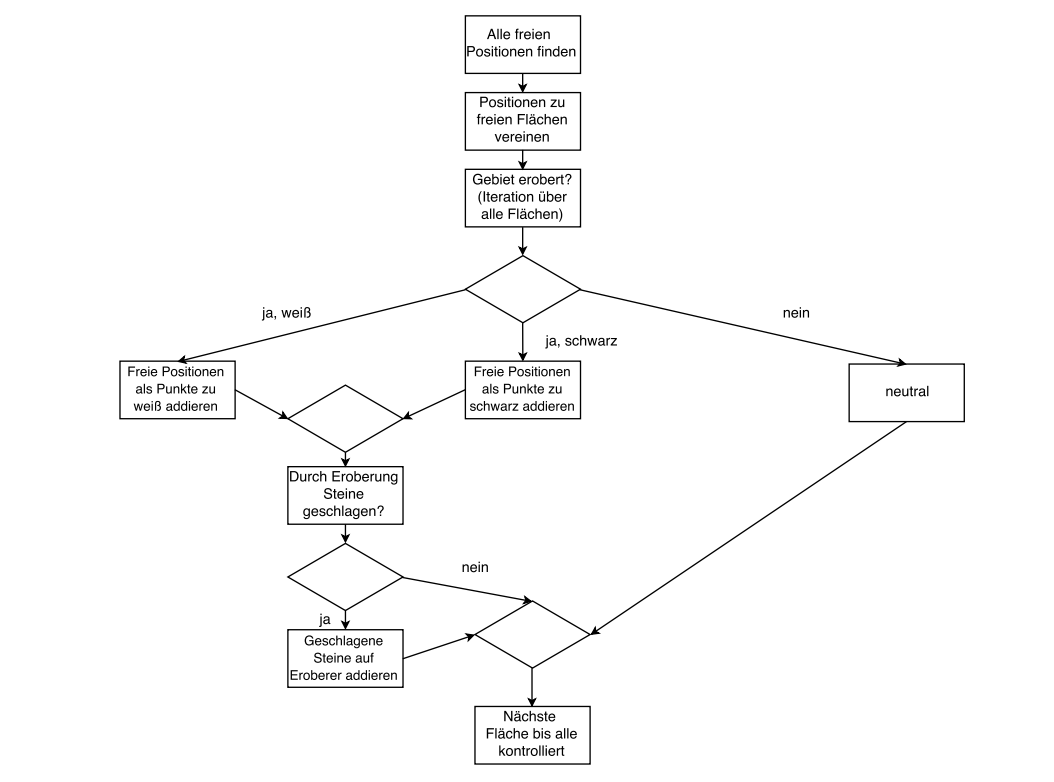
\includegraphics[width=1.1\textwidth]{images/AuswertungAblauf}
\caption{Ablaufdiagramm der Auswertung}
\end{figure}
Die Auswertung startet mit der Suche nach allen freien Positionen auf dem Spielfeld. Diese freien Positionen werden zu freien Fl"achen (=Gebiete) zusammengefasst. Anschlie"send wird jede freie Fl"ache "uberpr"uft, ob die Fl"ache von einem Spieler erobert wurde. Diese Funktionalit"at wird in dem Kapitel Gebietszuweisen (\ref{sec:Gebietszuweisung}) genauer erl"autert. Wurde ein Gebiet von einem Spieler erobert, wird die Anzahl der freien Positionen zu den Punkten des Spielers hinzugef"ugt. Liegen in dem eroberten Gebiet Steine des Gegners, werden diese geschlagen und ebenfalls dem Spieler als Punkte hinzugef"ugt. F"ur das Finden der geschlagenen Steine wird das eroberte Gebiet mit den Steinen des Eroberes aufgef"ullt. F"ur diesen Prozess werden die Funktionen zum Setzen eines Steines benutzt, um geschlagene Steine zu finden. Diese Funktionen sind in dem Kapitel Stein setzen (\ref{sec:SteinSetzen}) genauer beschrieben. Wird keinem Spieler ein Gebiet zugeschrieben, ist es neutral und kein Spieler erh"alt Punkte.\\\\
Diese Pr"ufung wird mit allen freien F"lachen durchlaufen, um so den Gesamtspielstand zu bestimmen. Am Ende werden die erzielten Punkte in der Auswertung auf die geschlagenen Steine w"ahrend des Spiels aufaddiert und der Sieger bestimmt.
\begin{figure}[ht]
\centering 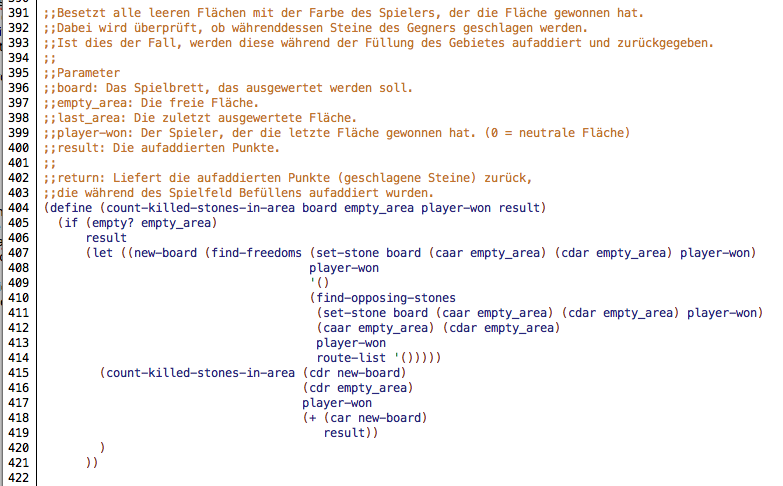
\includegraphics[width=1\textwidth]{images/CountKilledStones_code}
\caption{Z"ahlt die geschlagenen Steine aller eroberten Fl"ache}
\end{figure}
\newpage
\section{Gebietszuweisung}
\label{sec:Gebietszuweisung}
\begin{figure}[ht]
\newpage
\centering 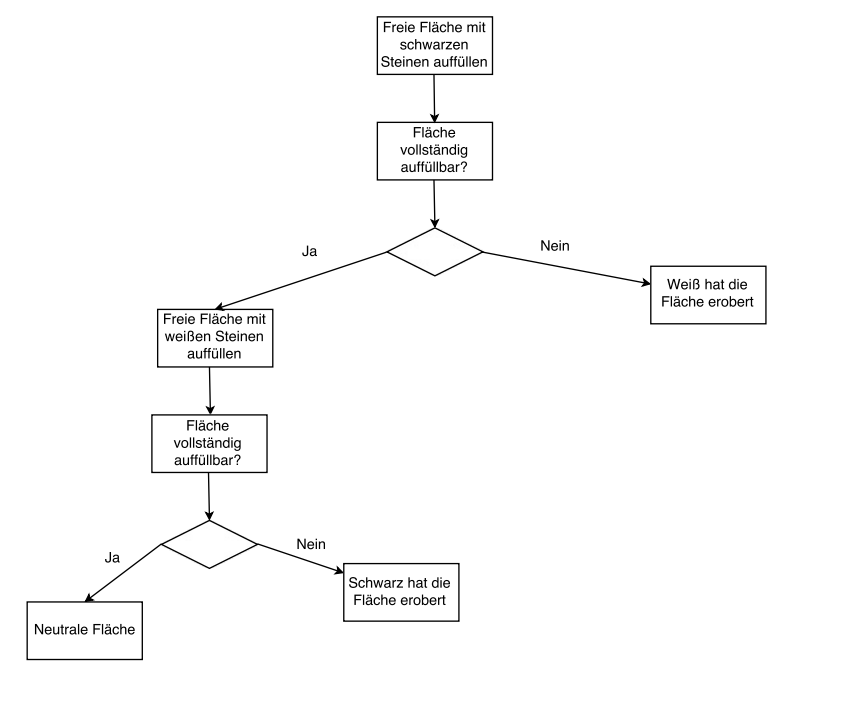
\includegraphics[width=1.1\textwidth]{images/GebietZuweisungAblauf}
\caption{Ablaufdiagramm der Gebietszuweisung}
\end{figure}
Um ein Gebiet einem Spieler zuzuweisen, muss gepr"uft werden, ob dieser das Gebiet erobert bzw. eingeschlossen hat. Auch hier werden die Funktionen der Stein setzen Funktionalit"at (\ref{sec:SteinSetzen}) verwendet. Das freie Fl"ache wird zuerst vollst"andig mit schwarzen Steinen aufgef"ullt. Ist die Fl"ache vollst"andig mit schwarzen Steinen auff"ullbar, dann ist Schwarz ein potentieller Eroberer der Fl"ache, weil sie nicht von Wei"s eingeschlossen ist. W"are dies der Fall, dann w"are die Fl"ache nicht vollst"andig auff"ullbar, weil Schwarz bei dem letzten Stein einen Selbstmord begehen w"urde. Dies ist aber in der Stein setzen Funktionalit"at (\ref{sec:SteinSetzen}) nicht erlaubt. Ist die Fl"ache also nicht vollst"andig auff"ullbar, dann ist wei"s der Eroberer dieser Fl"ache.\\\\
Davon ausgehend, dass Schwarz ein potentieller Eroberer ist, muss anschlie"send noch gepr"uft werden, ob Wei"s die Fl"ache ebenfalls auff"ullen darf. Darf Wei"s dies nicht, geh"ort die Fl"ache Schwarz. Darf Wei"s die Fl"ache ebenfalls komplett auff"ullen, ist die Fl"ache neutral, weil sie somit von keiner Farbe erobert ist.
\begin{figure}[ht]
\centering 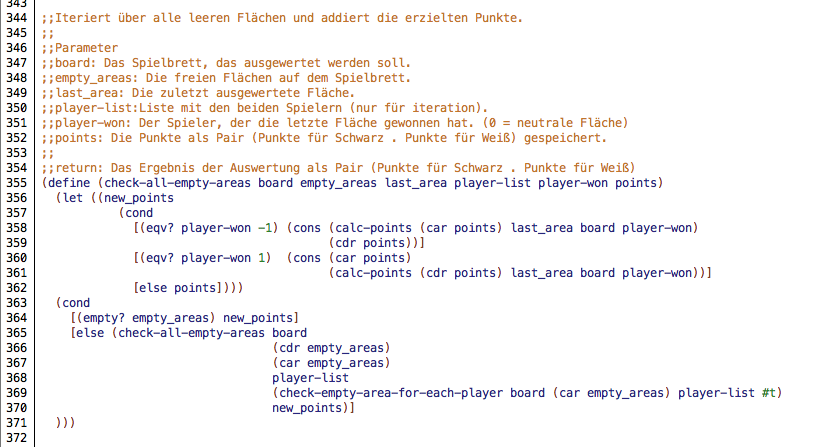
\includegraphics[width=1.1\textwidth]{images/checkAllAreas_code}
\caption{Pr"uft alle leeren Fl"achen auf eine Eroberung und addiert die freien eroberten Positionen zu den Punkten hinzu}
\end{figure}
\chapter{Beispiele}
\section{Erlaubter Selbstmord}
\begin{figure}[ht]
\centering 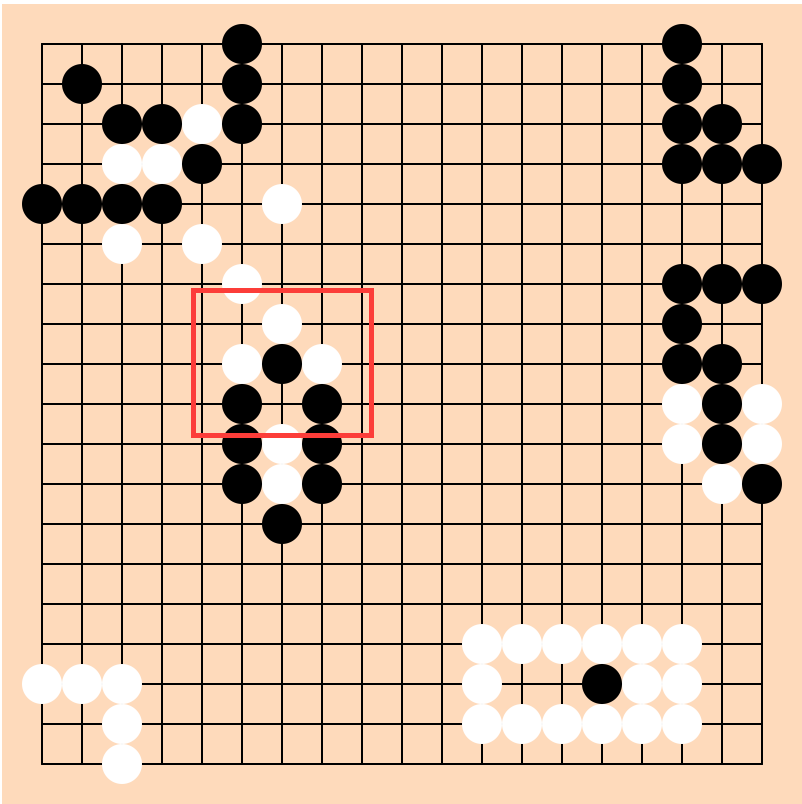
\includegraphics[width=0.4\textwidth]{images/VorErlSelbstmord}
\caption{Spielbrett vor erlaubten Selbstmord}
\end{figure}
\begin{figure}[ht]
\centering 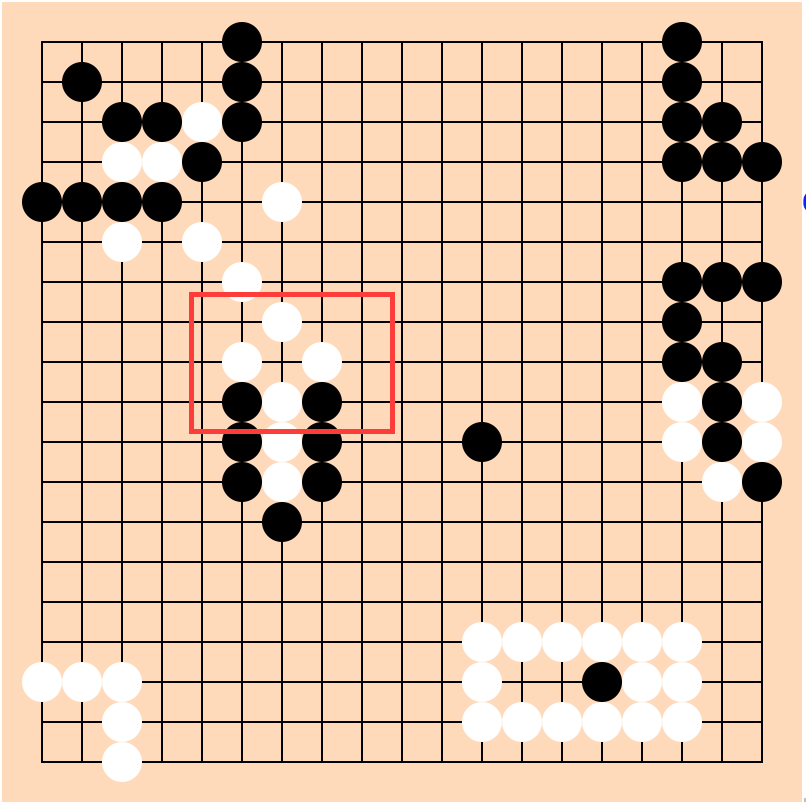
\includegraphics[width=0.4\textwidth]{images/NachErlSelbstmord}
\caption{Spielbrett nach dem erlaubten Selbstmord}
\end{figure}
\newpage
\section{Auswertung}
\begin{figure}[ht]
\centering 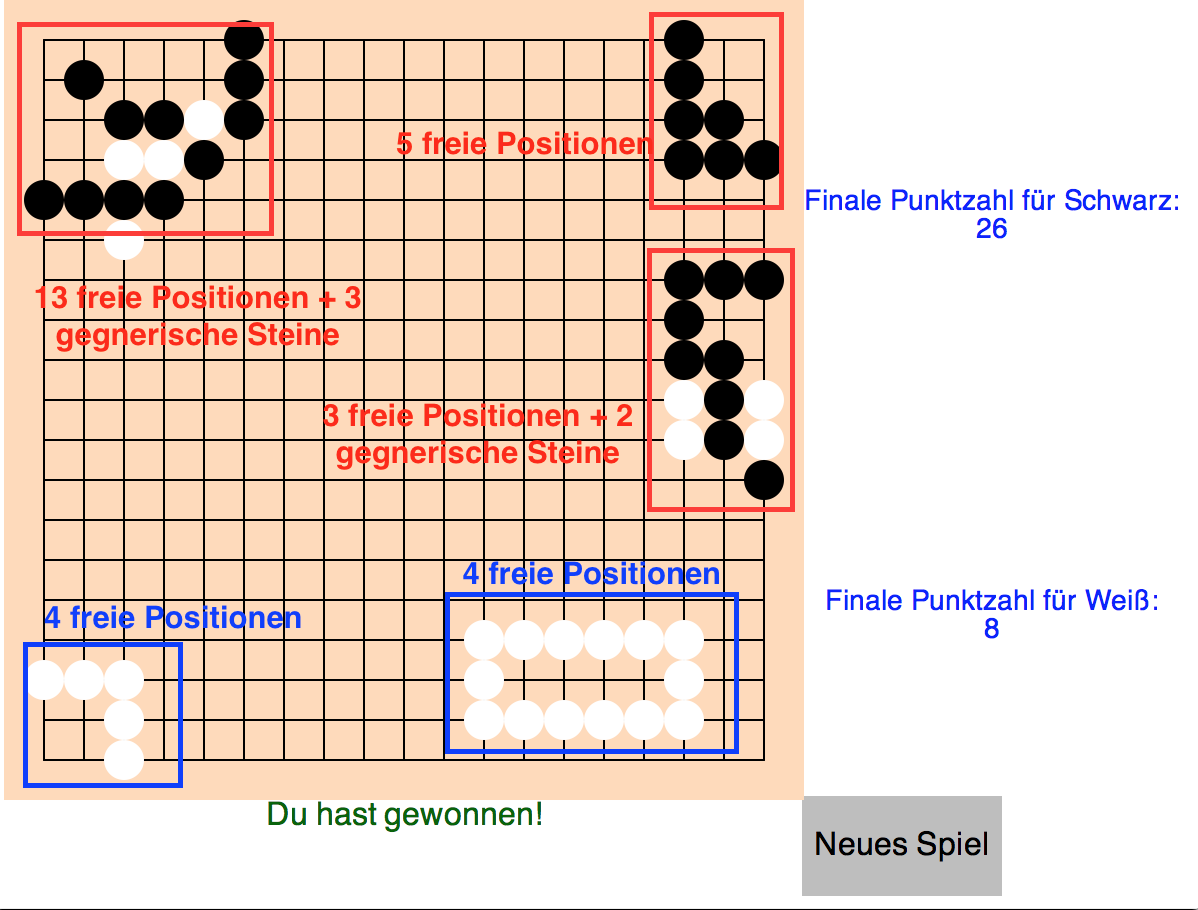
\includegraphics[width=1.2\textwidth]{images/Auswertung}
\caption{Beispielhafte Auswertung}
\end{figure}
\chapter{ToDo's}
\section{Dateiverarbeitung (go\_datei.rkt)}
Dieses Modul l"adt aus einer Spielstand-Datei den aktuellen Spielstand und gibt diesen als World (\ref{sec:World}) zur"uck. Ebenfalls kann dieses Modul einen Spielstand in die Datei schreiben. Die Datei enth"alt folgende Informationen:

\begin{enumerate}
\item Belegung des Spielfeldes (\ref{sec:Spielfeld})
\item Anzahl geschlagener Steine (schwarz . wei"s)
\item Der Spieler, der am Zug ist
\item Passstatus des vorherigen Spielers
\end{enumerate}

\section{Bug in Auswertung}
Aufgrund der hohen Komplexit"at der Auswertung war keine Zeit mehr einen Sonderfall in der Auswertung zu behandeln. Dieser tritt auf wenn eine eroberte Fl"ache durch gegnerische Steine unterbrochen wird (Abb. 6.1). Die Funktion, die die leeren Fl"achen sucht, erkennt dieses Gebiet als zwei leere Fl"achen, die von keiner Partei erobert wurden. Normalerweise muss bei der Auswertung erkannt werden, dass es sich nur um eine eroberte Fl"ache handelt und die gegnerischen Steine m"ussen geschlagen werden.
\begin{figure}[ht]
\centering 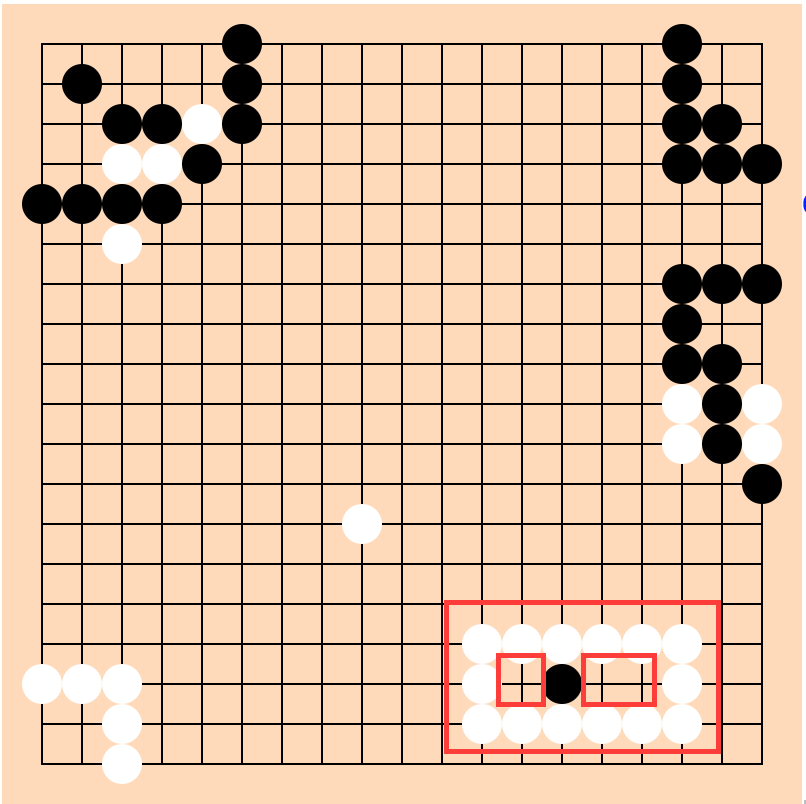
\includegraphics[width=0.3\textwidth]{images/AuswertungBug}
\caption{Spielbrett nach dem Schlagen des Steines}
\end{figure}
L"osungsansatz:\\
Es m"ussen drei Bedienungen gepr"uft werden, damit zwei getrennte Fl"achen als gemeinsame erkannt werden mu"ssen:
\begin{enumerate}
\item Beide Fl"achen d"urfen einzeln noch nicht erobert sein
\item Sie m"ussen "uber gegnerische Steine miteiander verbunden sein
\item Gemeinsam mit den gegnerischen Steinen muss die Fl"ache als erobert gelten
\end{enumerate}
Treten alle drei F"alle ein, d"urfen die leeren Fl"achen als gemeinsame betrachtet werden. Dann bekommt der Eroberer sowohl die Punkte f"ur die leeren Positionen als auch die Punkte f"ur die geschlagenen Steine.\\
Diese "Anderung muss in der Spiellogik implementiert werden, bevor die eigentliche Auswertung startet. Dann m"ussen alle gefundenen freien Fl"achen gepr"uft werden, ob sie zusammen geh"oren und anschlie"send in der Auswertung auch als gemeinsame Fl"ache betrachtet werden. Wir erachten den Aufwand als erheblich.

\end{document}
